\chapter{Introducción}

Consideremos un alfabeto finito, y sea $b$ la
cantidad de símbolos de este alfabeto.
Los collares ---o palabras circulares--- de
De Bruijn de orden $n$ son aquellas en las que todas las palabras de longitud
$n$ aparecen exactamente una vez.
Los collares de De Bruijn de orden $n$ tienen longitud $b^n$.
Nicolaas~Govert de~Bruijn \cite{de-bruijn-combinatorial-problem}
dio esta definición al mismo tiempo que los caracterizó como circuitos eulerianos
en los llamados grafos de De Bruijn, y contó cuántos hay.

Recientemente Alvarez, Becher, Ferrari y Yuhjtman \cite{alvarez-perfect-necklaces}
presentaron una generalización de los collares de De Bruijn,
que se llaman \emph{collares perfectos}.
Una collar es \emph{perfecto} de orden $(n,m)$ si todas las palabras 
de longitud $n$ ocurren exactamente $m$ veces, y todas ellas en distintas
posiciones módulo~$m$.
Los collares perfectos de orden $(n,m)$ tienen longitud $mb^n$.
En \cite{alvarez-perfect-necklaces} los collares perfectos están
caracterizados como circuitos eulerianos en los llamados grafos astutos,
dándose una fórmula para la cantidad de collares perfectos de orden $(n,m)$.

Becher y Carton \cite{becher-nested-perfect} definieron las
\emph{secuencias perfectas anidadas}; las mismas son palabras lineales ---no
circulares--- que, miradas circularmente, son collares perfectos de orden $(n,m)$
y, además, cuando $n>1$, son la concatenación de $b$ secuencias perfectas
anidadas de orden $(n-1, m)$.
En \cite{becher-nested-perfect} las secuencias perfectas anidadas son
caracterizadas como el resultado de una transformación lineal que puede
obtenerse a partir del triángulo de Pascal. Este trabajo también cuenta la
cantidad de secuencias perfectas anidadas $(n,m)$ sobre un alfabeto binario
siempre que $m$ es potencia de $2$.

Becher y Carton definieron las \emph{secuencias maravillosas anidadas}
de orden $(n,m)$ soltando la restricción de que las $m$ ocurrencias debieran
ocurrir en posiciones distintas módulo $m$, y dejaron abierta la pregunta de si
existen o no las secuencias maravillosas anidadas que no son perfectas anidadas.

Emprendimos este trabajo con el objetivo de responder la pregunta formulada por
Becher y Carton de si existen secuencias maravillosas anidadas que no son
perfectas anidadas.
En caso de responder positivamente, nos propusimos dar métodos de construcción
que permitieran obtener secuencias de estas características, con el objetivo
de máxima de contar la cantidad de secuencias maravillosas anidadas de orden
$(n,m)$ y, en caso de que esto no fuera posible, de poder brindar ejemplos que
garantizaran su existencia.

Llegamos a una respuesta rotundamente afirmativa siempre que $m$ sea
divisible por $b^{n-1}$. Para estos casos, definimos una subfamilia de las
secuencias maravillosas anidadas que llamamos \emph{autosimilares}. Cabe señalar
aquí que, dada su definición recursiva, toda secuencia maravillosa anidada
de orden $(n,m)$ es la concatenación de muchas secuencias maravillosas anidadas
de orden $(1,m)$. Una secuencia \emph{autosimilar} es aquella en la que todas
estas secuencias de orden mínimo ---a las que llamamos \emph{átomos}---
son iguales. Bajo las condiciones recién
mencionadas, demostramos que las secuencias maravillosas anidadas autosimilares
existen, que ninguna de ellas es perfecta anidada, y presentamos una fórmula
cerrada para su cantidad.

Podemos notar aquí que, para entrar dentro del caso recién presentado,
el valor de $n$ debe ser relativamente pequeño comparado con el de $m$;
en particular, $m \geq b^{n-1}$, por lo que $n$ debe ser a lo sumo del orden
del logaritmo de $m$ en base $b$.

En el otro extremo, se encuentran las duplas $(n,m)$ para las que $n$ es grande
en comparación con $m$. Para el caso de un alfabeto binario,
si $n$ es mayor que $2m$, demostramos que no es
posible encontrar secuencias maravillosas anidadas; si bien conjeturamos que
las mismas dejan de existir tan pronto como $n$ supera a $m + 1$.

Para los valores de $n$ y $m$ que quedan en medio de estos casos,
conjeturamos que las secuencias maravillosas anidadas existen. El abordaje de
estos casos lo realizamos mediante un análisis computacional, fijando un
alfabeto binario. Si bien el tamaño de las secuencias crece muy rápidamente al
incrementar $n$, dificultando el estudio de valores grandes de los parámetros,
los casos que sí es posible estudiar nos permiten extraer conclusiones
interesantes. En particular, podemos dar ejemplos de secuencias maravillosas
anidadas que no son perfectas anidadas para varios valores de $n$ y $m$, y
conjeturar que la cantidad de las primeras es considerablemente superior a la
de las últimas.

Un interés de las secuencias maravillosas anidadas es que se pueden usar
para construir secuencias normales en el sentido de Borel, que posiblemente
tienen la propiedad de converger a la normalidad muy rápidamente.
Suponemos que la velocidad de convergencia es la misma que la de la secuencia
de Levin \cite[Teorema 2]{levin-discrepancy-estimate}, la máxima conocida por
el momento.

El resto de este documento se estructura de la siguiente manera. El Capítulo
\ref{chapter:preliminaries} hace una introducción más rigurosa de las definiciones
involucradas en este trabajo, la notación empleada, y los resultados previos
que resultan relevantes. En el Capítulo \ref{chapter:autosimilar-sequences}
se presentan las secuencias autosimilares y se demuestra su existencia para
los valores de $n$ y $m$ antes mencionados, presentando una fórmula para su
cantidad. El Capítulo \ref{chapter:examples-and-conjectures} brinda un
análisis de la existencia de secuencias maravillosas anidadas para distintas
combinaciones de $n$ y $m$, integrando los resultados del capítulo anterior
con los datos obtenidos a partir del estudio computacional de las mismas.

\newpage

\chapter{Secuencias maravillosas anidadas}
\label{chapter:preliminaries}

Para comenzar, presentamos algunas definiciones sobre secuencias que son
esenciales para comprender este trabajo, como así también algunos detalles
de la notación que utilizamos a lo largo del mismo.

Sea $\alphabet$ un alfabeto fijo de $b$ símbolos, con $b \geq 2$. En los
ejemplos que brindamos a lo largo de este trabajo consideramos el alfabeto
$\alphabet = \lbrace 0, 1 \rbrace$, a menos que se indique lo contrario.
Llamamos \emph{palabra} o \emph{cadena} a una secuencia finita de caracteres
tomados de este alfabeto.
Para referirnos a las posiciones que ocupan los caracteres dentro de una
palabra, las numeramos comenzando en $1$.

Definimos la función de rotación $\sigma: \alphabet^* \to \alphabet^*$ como
una transformación biyectiva que quita el último carácter de una palabra y lo
coloca al principio. Es decir,
\[ \sigma(\alpha_1\dots\alpha_{n-1}\alpha_n) =
	\alpha_n\alpha_1\dots\alpha_{n-1}. \]

La aplicación sucesiva de la función de rotación divide a las palabras en clases
de equivalencia, que llamamos \emph{collares}. Un collar es, entonces, el
conjunto de todas las rotaciones posibles de una palabra, y lo notamos usando
corchetes:
\[ \neck{w} = \lbrace \sigma^{n}(w) : n \in \nats_0 \rbrace. \]
Por ejemplo,
\[ \neck{11100} = \lbrace 11100, 01110, 00111, 10011, 11001 \rbrace; \]
\[ \neck{00000} = \lbrace 00000 \rbrace. \]
Un collar puede pensarse como una ``palabra circular'', donde no importa
cuál de los caracteres es el primero. A cada una de las palabras que forman
parte de un collar la llamamos un \emph{corte} del mismo.

El \emph{período} de una palabra $w$ es el menor $n > 0$ tal que
$\sigma^n(w) = w$. Por ejemplo, la cadena $11001100$ tiene período $4$,
mientras que $11001101$ tiene período $8$.
Notar que el período de una cadena necesariamente divide a su longitud.
Además, es igual a la cantidad de cortes distintos que posee el collar al que
pertenece la palabra.

Una \emph{subcadena} es una secuencia de caracteres consecutivos dentro de una
palabra. 
En ocasiones, decimos que una palabra \emph{aparece} en otra palabra
para referirnos a que es una subcadena. Por ejemplo, $101$ y $1001$ aparecen en
(o son subcadenas de) la palabra $01010011$. Decimos que una palabra
\emph{aparece circularmente} en otra si aparece en alguna palabra del collar
correspondiente. Por ejemplo, $110$ no aparece en la palabra anterior, pero sí
aparece circularmente. En este caso, también podemos decir directamente que
la palabra aparece en el collar; en el ejemplo anterior, diríamos que $110$
aparece en $\neck{01010011}$.

\section{Collares y secuencias de De Bruijn}

En \cite{de-bruijn-combinatorial-problem}, Nicolaas G. de Bruijn realizó un detallado estudio de una clase
de collares que han pasado a ser conocidos con su nombre.

\begin{definition}[Collar de De Bruijn]
	Un \emph{collar de De Bruijn} de orden $n$ (o collar $n$-de De Bruijn) es un collar
	de longitud $b^n$ en el que cada una de las posibles palabras de longitud $n$ 
	aparece exactamente una vez.
\end{definition}

\begin{examples}\ %
	\begin{itemize}
		\item El collar $\neck{11000101}$ es un collar de De Bruijn de orden $3$.
		\item El collar $\neck{0101100111101000}$ es un collar de De Bruijn de orden $4$.
	\end{itemize}
\end{examples}

De Bruijn presenta una bonita caracterización de estos collares como circuitos
en una familia de digrafos que ha dado en conocerse como digrafos de De Bruijn.
El digrafo de De Bruijn de orden $n$ tiene como vértices todas las posibles
palabras de longitud $n$; existe una arista entre dos palabras si los últimos
$n-1$ caracteres de la primera coinciden con los primeros $n-1$ caracteres de la
segunda. Utilizamos la notación $G_n$ para referirnos al digrafo de De Bruijn
de orden $n$.

\begin{figure}[h] \centering
	\begin{tabular}{ccc}
		\begin{tabular}{c}
			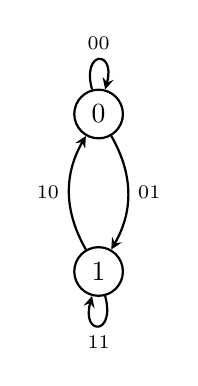
\begin{tikzpicture}[->,>=stealth,auto,node distance=2cm,
				every loop/.style={},thick,main node/.style={circle,draw}]
			
			\node[main node] (0) {0};
			\node[main node] (1) [below of=0] {1};
			
			\draw[every node/.style={font=\scriptsize}]
			(0) edge [bend left] node {01} (1)
					edge [loop above] node {00} (0)
			(1) edge [bend left] node {10} (0)
					edge [loop below] node {11} (1);
			\end{tikzpicture}
		\end{tabular} &

		\begin{tabular}{c}
			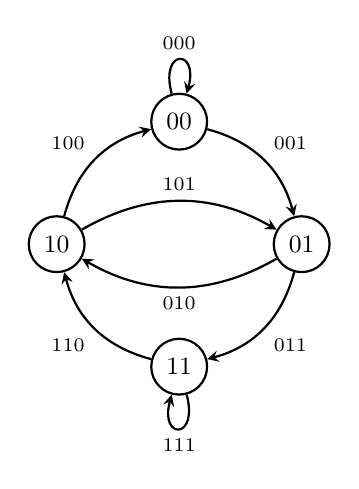
\begin{tikzpicture}[->,>=stealth,auto,node distance=2.2cm,
				every loop/.style={},thick,main node/.style={circle,draw,font=\small}]
			
			\node[main node] (00) {00};
			\node[main node] (01) [below right of=00] {01};
			\node[main node] (10) [below left of=00] {10};
			\node[main node] (11) [below right of=10] {11};
			
			\draw[every node/.style={font=\scriptsize}]
			(00) edge [loop above] node {000} (00)
					edge [bend left] node {001} (01)
			(01) edge [bend left] node {011} (11)
					edge [bend left] node {010} (10)
			(10) edge [bend left] node {100} (00)
					edge [bend left] node {101} (01)
			(11) edge [bend left] node {110} (10)
					edge [loop below] node {111} (11);
			\end{tikzpicture}
		\end{tabular} &

		\begin{tabular}{c}
			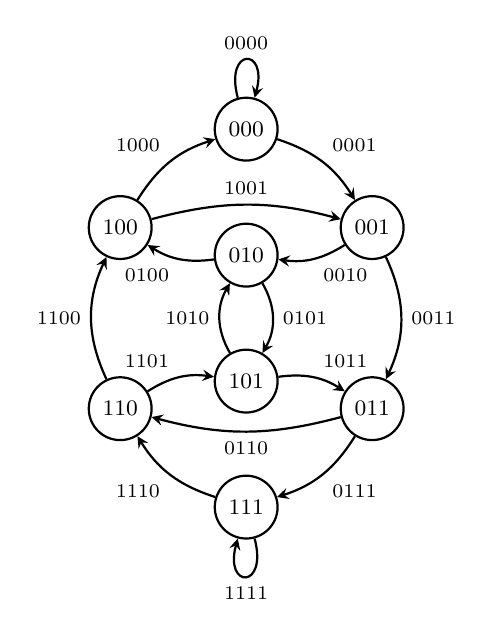
\begin{tikzpicture}[->,>=stealth,auto,node distance=1.6cm,
				every loop/.style={},thick,main node/.style={circle,draw,font=\footnotesize}]
			
			\node[main node] (000) {000};
			\node[main node] (010) [below of=000] {010};
			\node[main node] (101) [below of=010] {101};
			\node[main node] (111) [below of=101] {111};
			
			\node[main node] (001) [right of=010,yshift=.35cm] {001};
			\node[main node] (100) [left of=010,yshift=.35cm] {100};
			\node[main node] (011) [right of=101,yshift=-.35cm] {011};
			\node[main node] (110) [left of=101,yshift=-.35cm] {110};
			
			\draw[every node/.style={font=\scriptsize}]
			(000) edge [loop above] node {0000} (000)
						edge [bend left=20] node {0001} (001)
			(001) edge [bend left=20] node {0010} (010)
						edge [bend left=25] node {0011} (011)
			(010) edge [bend left=20] node {0100} (100)
						edge [bend left] node {0101} (101)
			(011) edge [bend left=15] node {0110} (110)
						edge [bend left=20] node {0111} (111)
			(100) edge [bend left=20] node {1000} (000)
						edge [bend left=15] node {1001} (001)
			(101) edge [bend left] node {1010} (010)
						edge [bend left=20] node {1011} (011)
			(110) edge [bend left=25] node {1100} (100)
						edge [bend left=20] node {1101} (101)
			(111) edge [bend left=20] node {1110} (110)
						edge [loop below] node {1111} (111);
			\end{tikzpicture}
		\end{tabular} \\
		$G_1$ & $G_2$ & $G_3$
	\end{tabular}
	\caption{Digrafos de De Bruijn de orden $1$, $2$ y $3$
		para $\alphabet = \lbrace 0, 1 \rbrace$.}
\end{figure}

Cada collar de De Bruijn de orden $n$ se corresponde unívocamente con un circuito
hamiltoniano en el digrafo $G_n$, es decir, un camino cerrado que visita cada
vértice exactamente una vez. El collar se conforma concatenando en orden
el primer carácter de cada uno de los vértices visitados por el circuito.

Una propiedad muy interesante de la familia de digrafos de De Bruijn es que
cada $G_n$ es el grafo de línea de $G_{n-1}$; es decir, $G_n$ puede
construirse tomando como vértices el conjunto de aristas de $G_{n-1}$ y
colocando una arista entre cada par de vértices si las aristas correspondientes
en $G_{n-1}$ son adyacentes. Esto quiere decir que los circuitos hamiltonianos
en $G_n$ se corresponden con circuitos eulerianos en $G_{n-1}$, esto es,
caminos cerrados que utilizan cada arista exactamente una vez.

De Bruijn utiliza esta naturaleza recursiva de la familia de digrafos $G_n$
para demostrar una fórmula cerrada para la cantidad de collares de De Bruijn
de orden $n$ existentes, que en el caso de un alfabeto binario es exactamente
$\frac{2^{2^{n-1}}}{2^n}$. Este resultado fue luego generalizado en
\cite{van-aardenne-ehrenfest-circuits-and-trees} para alfabetos de tamaño arbitrario,
donde la cantidad de collares es $\frac{(b!)^{b^{n-1}}}{b^n}$.

Cabe señalar que, debido a sus características, la forma más natural de
presentar la definición de los collares de De Bruijn es justamente en términos
de collares, o palabras circulares. No obstante ---y esta situación se repite
para otras definiciones similares que aparecen más adelante en este trabajo---,
en ocasiones interesa tener en cuenta cada corte particular de un collar como
un elemento distinto. Por eso, en adelante, utilizaremos el término
\emph{secuencia de De Bruijn} para referirnos a un corte de un collar de De
Bruijn\footnote{Queremos hacer énfasis en este punto, ya que el término
\emph{secuencia de De Bruijn} es utilizado de forma ambigua en la literatura.
Para algunos autores, una secuencia de De Bruijn de orden $n$ es una secuencia
de longitud $b^n + n - 1$, donde cada palabra posible de longitud $n$ aparece
exactamente una vez, sin considerar apariciones circulares. Notar, sin embargo,
que las secuencias de De Bruijn así entendidas están en correspondencia uno a
uno con las que definimos aquí, con la única diferencia de que en ellas los
primeros $n-1$ caracteres aparecen repetidos al final.}.

¿Cuántas secuencias de De Bruijn de orden $n$ existen para cada $n$? Se puede notar que
el período de una secuencia $n$-de De Bruijn es necesariamente igual a su
longitud, $b^n$; de lo contrario, la palabra de longitud $n$ con la que comienza
volvería a aparecer más adelante. Luego, cada collar $n$-de De Bruijn tiene
$b^n$ cortes distintos, con lo cual la cantidad de secuencias $n$-de De Bruijn
es exactamente $(b!)^{b^{n-1}}$.

\section{El teorema \BEST{}}

El teorema \BEST{} es un resultado en teoría de grafos que permite determinar la
cantidad de circuitos eulerianos en un multidigrafo. Recibe su nombre por las
iniciales de sus descubridores, De Bruijn, Van Aardenne-Ehrenfest, Smith y
Tutte.

\begin{theorem*}[\BEST{}, \cite{van-aardenne-ehrenfest-circuits-and-trees}]
	Sea $G$ un multidigrafo euleriano con vértices $v_1, \dots, v_n$.
	La cantidad de circuitos eulerianos en $G$ está dada por
	\[ \operatorname{ec}(G) = t_k \prod_{i=1}^n (d_i - 1)!, \]
	donde $d_i$ es el grado de salida de $v_i$ y $t_k$ es la cantidad de árboles
	generadores de $G$ orientados hacia un vértice $v_k$ arbitrario.
\end{theorem*}

Para obtener la cantidad de árboles generadores en un multidigrafo euleriano,
puede usarse a su vez el teorema de Kirchoff (también conocido como teorema
Matrix-Tree), que permite calcularla
a partir de su \emph{matriz laplaciana}, definida como
\[ \laplacian(G) = \left\lbrace \begin{array}{ll}
	d_i - d_{ii} & \text{si $i = j$} \\
	-d_{ij}       & \text{si $i \neq j$}
\end{array} \right\rbrace_{i,j = 1,\dots,n}, \]
donde $d_i$ es el grado de salida de $v_i$ y $d_{ij}$ es la cantidad de
aristas que van de $i$ a $j$.

\begin{theorem*}[Kirchoff, ver \cite{farrell-multi-eulerian-tours}]
	Sea $G$ un multidigrafo con vértices $v_1, \dots, v_n$. La cantidad $t_i$
	de árboles generadores orientados hacia un vértice $v_i$ es el $i$-ésimo
	cofactor de la matriz $\laplacian(G)$, es decir,
	\[ t_i = \operatorname{det}(\laplacian_i(G)), \]
	siendo $\laplacian_i(G)$ la matriz que se obtiene al omitir la $i$-ésima fila
	y la $i$-ésima columna de $\laplacian(G)$.
\end{theorem*}

En multidigrafos eulerianos, el vértice que se elija resulta irrelevante, ya
que la cantidad de árboles generadores hacia cualquiera de ellos es invariante;
en otras palabras, todos los cofactores de $\laplacian(G)$ son iguales. En
el caso concreto del digrafo de De Bruijn de orden $n$, tenemos que
\cite{van-aardenne-ehrenfest-circuits-and-trees} para cualquier
$k = 1, \dots, 2^n$,
\[ t_k = \frac{b^{b^{n}}}{b^{n+1}}, \]
lo cual, junto al hecho de que posee exactamente $b^n$ vértices y el grado de
salida de todos ellos es exactamente $b$, permite utilizar el teorema \BEST{} para
contabilizar la cantidad de circuitos eulerianos:
\begin{align*}
	\operatorname{ec}(G_n) &= t_k \prod_{i=1}^{b^n} (d_i - 1)! \\
		&= \frac{b^{b^{n}}}{b^{n+1}} \left((b - 1)!\right)^{b^n} \\
		&= \frac{(b!)^{b^{n}}}{b^{n+1}}.
\end{align*}

Notar que esta fórmula se corresponde exactamente con la dada en la sección
anterior para la cantidad de collares de De Bruijn de orden $n + 1$.

\section{Secuencias maravillosas}

A continuación presentamos una generalización de las secuencias de De Bruijn,
que denominaremos \emph{secuencias maravillosas}.

\begin{definition}[Secuencia maravillosa]
Sea un alfabeto de $b$ símbolos.
Un \emph{collar $(n,m)$-maravilloso} es un collar de longitud $mb^n$
en el que cada una de las posibles palabras de longitud $n$ aparece
exactamente $m$ veces.

Una \emph{secuencia $(n,m)$-maravillosa} es un corte de un collar
$(n,m)$-maravilloso.
\end{definition}

\begin{examples}\ %
	\begin{itemize}
		\item Las siguientes secuencias son $(2,4)$ y $(3,3)$-maravillosas, respectivamente:
		\[ 1110000111010010; \qquad 000111110110110100100100. \]
		\item Todas las secuencias de De Bruijn de orden $n$ son ejemplos de secuencias
		$(n,1)$-maravillosas.
	\end{itemize}
\end{examples}

Una pregunta inmediata que surge de esta definición es cómo puede extenderse a
los collares maravillosos la caracterización como circuitos eulerianos
presentada para los collares de De Bruijn, y si es posible utilizar este enfoque
para determinar la cantidad de secuencias maravillosas existentes para cada valor
de $n$ y $m$, lo cual resulta de especial interés más adelante en este
trabajo.

Un enfoque posible consiste en definir una familia de \emph{multidigrafos de De
	Bruijn}.
Llamamos multidigrafo de De Bruijn de orden $n$ y grado $m$ al multidigrafo
$G_n^m$ que se obtiene a partir del digrafo de De Bruijn de orden $n$ si se
replica $m$ veces cada arista.
Con esta definición, es inmediato comprobar que todo circuito euleriano en
$G_n^m$ (o hamiltoniano en $G_{n+1}^m$) determina de manera unívoca un collar
$(n+1, m)$-maravilloso.
Recordemos que cada arista de $G_n$ puede asociarse con una palabra distinta de
longitud $n+1$; como en $G_n^m$ existen $m$ copias de cada arista, una
secuencia obtenida a partir de un circuito euleriano contendrá cada una de
estas palabras exactamente $m$ veces.


\begin{figure}[h] \centering
	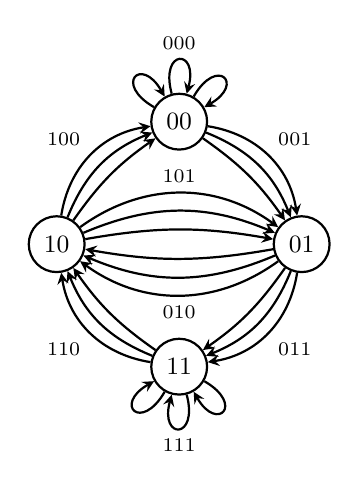
\begin{tikzpicture}[->,>=stealth,auto,node distance=2.2cm,
		every loop/.style={},thick,main node/.style={circle,draw,font=\small}]
	
	\node[main node] (00) {00};
	\node[main node] (01) [below right of=00] {01};
	\node[main node] (10) [below left of=00] {10};
	\node[main node] (11) [below right of=10] {11};
	
	\draw[every node/.style={font=\scriptsize}]
	(00) edge [in=30, out=60, loop] (00)
	     edge [loop above] node {000} (00)
	     edge [in=120, out=150, loop] (00)
	     edge [bend left=36] node {001} (01)
	     edge [bend left=23] (01)
	     edge [bend left=10] (01)
	(01) edge [bend left=36] node {011} (11)
	     edge [bend left=23] (11)
	     edge [bend left=10] (11)
	     edge [bend left=36] node {010} (10)
	     edge [bend left=23] (10)
	     edge [bend left=10] (10)
	(10) edge [bend left=36] node {100} (00)
	     edge [bend left=23] (00)
	     edge [bend left=10] (00)
	     edge [bend left=36] node {101} (01)
	     edge [bend left=23] (01)
	     edge [bend left=10] (01)
	(11) edge [bend left=36] node {110} (10)
	     edge [bend left=23] (10)
	     edge [bend left=10] (10)
	     edge [in=210, out=240, loop] (11)
	     edge [loop below] node {111} (11)
	     edge [in=300, out=330, loop] (11);
	\end{tikzpicture}
	\caption{Multidigrafo de De Bruijn de orden $2$ y grado $3$
		para $\alphabet = \lbrace 0, 1 \rbrace$.}
\end{figure}

No obstante, esto no vale a la inversa, ya que si $m > 1$, todo collar
$(n+1,m)$-maravilloso se corresponde con más de un ciclo euleriano en $G_n^m$.
Esto se debe a que las $m$ apariciones de una palabra de longitud $n + 1$ en un
collar son indistinguibles, por lo que las $m$ aristas respectivas pueden ser
permutadas, obteniendo un nuevo ciclo euleriano que se corresponde con el mismo
collar.
Concretamente, como existen $m! $ maneras de permutar cada conjunto de $m$
aristas, se tiene un total de $m!b^{n+1}$ maneras distintas de
representar un collar $(n+1,m)$-maravilloso con un circuito euleriano.

Si se tiene este hecho en consideración, es posible aplicar el teorema \BEST{}
para contabilizar la cantidad de circuitos eulerianos en los multidigrafos de
De Bruijn y así obtener una fórmula cerrada para la cantidad de collares
maravillosos.
Sin embargo, si lo que se desea contar son las secuencias maravillosas ---en
lugar de los collares---, surge una nueva dificultad, ya que a diferencia de los
collares de De Bruijn, el período de un collar maravilloso no es invariante, es
decir, la cantidad de secuencias distintas que pueden obtenerse realizando
cortes a un collar maravilloso es diferente para cada collar.

Si bien existen formas de incorporar este nuevo elemento en los cálculos,
por simplicidad, decidimos buscar un enfoque alternativo que
permitiera caracterizar directamente las secuencias maravillosas, utilizando la
noción de \emph{circuito $\pi$-euleriano} presentada por Farrell y Levine en
\cite{farrell-multi-eulerian-tours}.

\begin{definition}[Circuito $\pi$-euleriano, \cite{farrell-multi-eulerian-tours}]
	Sea $G$ un digrafo con vértices $v_1, \dots, v_n$, y sea $\pi \in
		\mathbb{N}^n$
	un vector con valores estrictamente positivos.
	Un circuito $\pi$-euleriano en $G$ es un circuito donde cada arista
	($v_i$, $v_j$) se utiliza exactamente $\pi_j$ veces.
\end{definition}

Esta noción generaliza la de circuito euleriano, ya que estos son circuitos
$\pi$-eulerianos con $\pi = (1, \dots, 1)$.
Partiendo de aquí, los autores presentan la siguiente generalización del
teorema \BEST{}.

\begin{theorem*}[\BEST{} generalizado, \cite{farrell-multi-eulerian-tours}]
	\label{prop:BEST-generalized}
	Sea $G$ un multidigrafo fuertemente conexo con vértices $v_1, \dots, v_n$, y
	sea $\pi \in \mathbb{N}^n$.
	Existen circuitos $\pi$-eulerianos en $G$ si y solo si
	\[ \laplacian(G) \cdot \pi = 0, \]
	en cuyo caso la cantidad de estos circuitos que comienzan con una arista $e$
	determinada es
	\[ \operatorname{ec}_\pi(G, e) = t_e
		\prod_{i=1}^n \frac{(d_i\pi_i - 1)! }{(\pi_i!)^{d_i-1}(\pi_i-1)!}, \]
	donde $d_i$ es el grado de salida de $v_i$, y $t_e$ es la cantidad de árboles
	generadores de $G$ orientados hacia la cola de $e$.
\end{theorem*}

El interés de esta generalización para nuestro problema particular radica en que
una secuencia $(n+1,m)$-maravillosa puede identificarse de forma unívoca con un
circuito $\pi$-euleriano en $G_n$ tomando $\pi = (m,\dots,m)$ y fijando cuál
será su arista inicial.
Esto nos permite enunciar y demostrar el siguiente resultado.

\begin{proposition}
	\label{proposition:marvellous-count}
	Sean $n, m > 0$.
	La cantidad de secuencias $(n,m)$-maravillosas es exactamente
	\[ \left( \frac{(bm)! }{(m!)^b} \right)^{b^{n-1}}. \]
\end{proposition}

\begin{proof}
	Consideramos primero el caso en que $n > 1$.
	En este caso, como se mencionó anteriormente, fijando $\pi = (m, \dots, m)$,
	basta con determinar la cantidad de circuitos $\pi$-eulerianos en $G_{n-1}$
	para cada una de las posibles elecciones de arista inicial.
	Sabemos que existen circuitos $\pi$-eulerianos en $G_{n-1}$, ya que se trata
	de un digrafo euleriano, por lo que basta con tomar un circuito euleriano y
	repetirlo $m$ veces para obtener un ejemplo.
	Es decir que, en virtud del teorema \BEST{} generalizado, la cantidad de
	secuencias maravillosas será igual a \[ \sum_e \operatorname{ec}_\pi(G_{n-1}, e) =
		\sum_e t_e \prod_{i=1}^{b^{n-1}} \frac{(d_i\pi_i - 1)!
		}{(\pi_i!)^{d_i-1}(\pi_i-1)!}, \] donde la suma se realiza sobre todas las
	aristas del digrafo $G_{n-1}$.

	Se sabe que la cantidad de aristas de $G_{n-1}$ es $b^n$; por otro lado,
	como ya se mencionó anteriormente, la
	cantidad de árboles generadores orientados hacia cualquiera de los vértices
	de $G_{n-1}$ es $\frac{b^{b^{n-1}}}{b^n}$, de donde se sigue que
	$\sum_{e} t_e = b^{b^{n-1}}$.
	Reemplazando en la expresión anterior, se obtiene \[ b^{b^{n-1}}
		\prod_{i=1}^{b^{n-1}} \frac{(d_i\pi_i - 1)! }{(\pi_i!)^{d_i-1}(\pi_i-1)!}.
	\]

	Dado que $G_{n-1}$ es un digrafo regular cuyos vértices tienen todos grado de
	salida $b$, y dado que $\pi_i = m$ para todo $i = 1, \dots, b^{n-1}$, la
	expresión anterior equivale a
	\begin{align*}
		b^{b^{n-1}} \left( \frac{(bm - 1)! }{(m!)^{b-1}(m-1)!} \right)^{b^{n-1}}
			&= \left( \frac{b (bm - 1)! }{(m!)^{b-1}(m-1)!} \right)^{b^{n-1}} \\
			&= \left( \frac{bm (bm - 1)! }{(m!)^{b-1}m(m-1)!} \right)^{b^{n-1}} \\
			&= \left( \frac{(bm)! }{(m!)^b} \right)^{b^{n-1}}.
	\end{align*}

	Resta demostrar el caso en que $n = 1$. Para esto, basta observar que una
	secuencia $(1,m)$-maravillosa es una secuencia de longitud $bm$ en donde
	cada uno de los $b$ símbolos del alfabeto aparece exactamente $m$ veces.
	Por lo tanto, para construir una de estas secuencias, en primer lugar es
	necesario seleccionar cuáles $m$ de entre las $bm$ posiciones corresponderán
	al primer símbolo; luego, cuáles $m$ de entre las $(b - 1)m$ posiciones
	restantes corresponderán al segundo símbolo; en tercer lugar, cuáles $m$ de
	entre las $(b - 2)m$ posiciones restantes corresponderán al tercer símbolo,
	y así sucesivamente. Es decir, la cantidad de formas distintas de construir
	una secuencia $(1,m)$-maravillosa puede expresarse como el siguiente producto
	de números combinatorios:
	\begin{align*}
		\prod_{i = 0}^{b - 1} \binom{(b - i)m}{m}
			&= \prod_{i = 0}^{b - 1} \frac{((b-i)m)!}{m!((b-i-1)m)!} \\
			&= \frac{(bm)!}{m!((b-1)m)!} \cdot
				\frac{((b-1)m)!}{m!((b-2)m)!} \cdot
				\frac{((b-2)m)!}{m!((b-3)m)!} \cdot \dots \cdot
				\frac{m!}{m!0!} \\
			&= \frac{(bm)!}{(m!)^b},
		\end{align*}
	lo cual es consistente con la fórmula presentada.
\end{proof}

\section{Secuencias maravillosas anidadas}

Las secuencias maravillosas que acabamos de presentar son primas cercanas de
las \emph{secuencias perfectas}.
Una secuencia $(n,m)$-perfecta es una secuencia de longitud $m b^n$ en la
que cada posible palabra de longitud $n$ aparece circularmente exactamente
$m$ veces, al igual que en las secuencias maravillosas, pero con la restricción
adicional de que cada una de estas apariciones se produce en una posición
distinta módulo $m$. Por ejemplo, la siguiente es una secuencia $(2,4)$-perfecta:
\[ 0000111001011011. \]

Puede verse una presentación de estas secuencias en \cite{alvarez-perfect-necklaces},
junto a una caracterización de las mismas en términos de una modificación
de los digrafos de De Bruijn, los denominados grafos astutos, y una fórmula
para su cantidad.

En \cite{becher-nested-perfect}, Becher y Carton definen las \emph{secuencias
perfectas anidadas}. Una secuencia $(n,m)$-perfecta anidada es una secuencia
perfecta de orden $(n,m)$ que además, si $n > 1$, es la concatenación de $b$
secuencias perfectas anidadas de orden $(n-1,m)$. Por ejemplo, la secuencia
recién mostrada no es $(2,4)$-perfecta anidada, ya que sus dos mitades no son secuencias
$(1,4)$-perfectas; notar que en $00001110$, la palabra $0$ aparece cinco veces,
mientras que la palabra $1$ aparece solo tres veces. Sin embargo, al rotarla
una posición, se obtiene el siguiente ejemplo de secuencia $(2,4)$-perfecta
anidada:
\[ 10000111\;00101101. \]

Los autores de \cite{becher-nested-perfect} brindan un método matricial que
permite generar todas estas secuencias basado en el triángulo
de Pascal, siempre y cuando se cumplan ciertas restricciones,
en particular que $b$ sea un número primo, $m$ una potencia de $2$ y $n \leq m$.
También brindan una fórmula cerrada para la cantidad de secuencias
$(n,m)$-perfectas anidadas en estos casos.

Todo esto motiva una definición análoga, pero considerando secuencias
maravillosas en lugar de perfectas: las \emph{secuencias maravillosas anidadas},
el principal objeto de estudio de este trabajo.

\begin{definition}
	Sea un alfabeto de $b$ símbolos.
	Una \emph{secuencia $(n,m)$-maravillosa anidada} es una secuencia de
	longitud $m b^n$ para la que se cumple simultáneamente que
	\begin{enumerate}
		\item es una secuencia $(n,m)$-maravillosa; y
		\item si $n > 1$, es la concatenación de $b$ secuencias
		      $(n-1,m)$-maravillosas anidadas.
	\end{enumerate}

	Alternativamente, una secuencia es $(n,m)$-maravillosa anidada si, para todo
	$n'$ tal que $1 \leq n' \leq n$, toda subsecuencia de longitud
	$m b^{n'}$ que comienza en una posición congruente a $1$ módulo
	$m b^{n'}$ es $(n',m)$-maravillosa.
\end{definition}

\begin{examples}
	Las siguientes secuencias son $(3,3)$, $(2,4)$ y $(1,5)$-maravillosas anidadas,
	respectivamente:
	\[ 000111\;011001\;000111\;101010; \]
	\[ 00010111\;10100110; \]
	\[ 0011101010. \]
\end{examples}

Una observación que podemos hacer a partir de esta definición es que, si miramos
el más profundo de sus niveles de anidación, cada secuencia $(n,m)$-maravillosa
anidada está conformada por la concatenación de $b^{n-1}$ secuencias
$(1,m)$-maravillosas anidadas, cada una de ellas de longitud $bm$. En otras
palabras, si fijamos un valor de $m$, todas las secuencias $(n,m)$-maravillosas
anidadas ---para cualquier valor de $n$--- están formadas por los mismos
``ladrillos'' básicos, las secuencias $(1,m)$-maravillosas anidadas. Para estas
secuencias utilizamos en adelante el nombre de $m$-átomos. Dado que cuando
$n = 1$ las definiciones de secuencia maravillosa y maravillosa anidada
conciden, los $m$-átomos son exactamente las secuencias $(1,m)$-maravillosas;
esto implica (según la Proposición \ref{proposition:marvellous-count})
que la cantidad de $m$-átomos es exactamente $\frac{(bm)!}{(m!)^b}$.

A modo ilustrativo, estos son los $20$ átomos de orden $3$ que existen para
$\alphabet = \lbrace 0, 1 \rbrace$:
\[
	\begin{array}{ccccc}
		\text{1. }000111 & \text{2. }001011 & \text{3. }001101 & \text{4. }001110 & \text{5. }010011 \\
		\text{6. }010101 & \text{7. }010110 & \text{8. }011001 & \text{9. }011010 & \text{10. }011100 \\
		\text{11. }100011 & \text{12. }100101 & \text{13. }100110 & \text{14. }101001 & \text{15. }101010 \\
		\text{16. }101100 & \text{17. }110001 & \text{18. }110010 & \text{19. }110100 & \text{20. }111000 \\
	\end{array}
\]
El ejemplo de secuencia $(3,3)$-maravillosa anidada presentado más arriba puede
pensarse, entonces, como la concatenación de los átomos 1, 8, 1 y 15, en ese
orden.

De las definiciones presentadas se desprende fácilmente que todas las secuencias
perfectas anidadas son maravillosas anidadas. Por lo tanto, la existencia de
secuencias maravillosas anidadas de orden $(n,m)$ está fuera de cuestión
siempre que existen secuencias $(n,m)$-perfectas anidadas. Ahora bien, en estos
casos, ¿existen secuencias maravillosas anidadas \emph{que no sean} perfectas
anidadas? Esta es la pregunta central que buscamos responder en lo que resta
de este trabajo.

\newpage

\chapter{Una familia maravillosa}
\label{chapter:autosimilar-sequences}

Esta sección tiene por objetivo brindar una demostración del siguiente teorema
de existencia, presentando un método constructivo para una familia particular
de secuencias maravillosas anidadas. Al igual que en la sección anterior,
$b$ hace referencia a la cantidad de símbolos del alfabeto, y los ejemplos
presentados son para el alfabeto $\alphabet = \lbrace 0, 1 \rbrace$.

\begin{theorem}
	\label{theorem:existence-autosimilar}
	Si $b^{n-1}$ divide a $m$, existen secuencias $(n,m)$-maravillosas anidadas
	que no son perfectas anidadas.
\end{theorem}

El primer paso para demostrar este teorema es presentar la familia de secuencias
para la que daremos un método constructivo; se trata de las que llamamos
\emph{secuencias autosimilares}.

\begin{definition}
	Una secuencia $x$ es $(n,m)$-\emph{autosimilar} si consiste en $b^{n-1}$
	repeticiones de una misma secuencia de longitud $bm$.
\end{definition}

\begin{example}
	La secuencia \[ 01110110\ 01110110\ 01110110\ 01110110 \] es
	$(3,4)$-autosimilar.
	La secuencia \[ 110000101011 \ 110000101011 \] es $(2,6)$-autosimilar; además,
	es $(2,6)$-maravillosa anidada.
\end{example}

Nos interesa estudiar las secuencias $(n,m)$-maravillosas anidadas que, además,
son autosimilares.
Podemos notar que las mismas consisten precisamente en la concatenación
de $b^{n-1}$ copias de un mismo $m$-átomo.

La proposición que enunciamos a continuación nos permite caracterizar a
las secuencias $(n,m)$-maravillosas anidadas autosimilares a
partir de una propiedad verificable los átomos que les dan origen.
Gracias a este resultado, podemos determinar para qué valores de $(n,m)$ existen
este tipo de secuencias, cuál es su cantidad, y presentar un método para su
construcción.

\begin{proposition}
	\label{proposition:autosimilar-nm-characterization}
	Sea $x = \omega^{b^{n-1}}$ una secuencia $(n,m)$-autosimilar.
	La secuencia $x$ es $(n,m)$-maravillosa anidada si y solo si $b^{n-1}$
	divide a $m$ y $\omega$
	es una secuencia $\left( n, \frac{m}{b^{n-1}} \right)$-maravillosa.
\end{proposition}

\begin{examples}\ %
	\begin{itemize}
		\item El $4$-átomo $01011100$ es $(1,4)$, $(2,2)$ y
		      $(3,1)$-maravilloso.
		      Por lo tanto, las siguientes tres secuencias son $(1,4)$, $(2,4)$ y
		      $(3,4)$-maravillosas anidadas, respectivamente.
		      \[ 01011100; \qquad 01011100\ 01011100; \qquad 01011100\
			      01011100\ 01011100\ 01011100.
		      \]
		\item El $4$-átomo $10001101$ es $(1,4)$ y $(2,2)$-maravilloso,
		      pero no $(3,1)$-maravilloso.
		      Por lo tanto, las siguientes dos secuencias son $(3,1)$ y $(3,2)$-maravillosas
		      anidadas, respectivamente.
		      \[ 10001101; \qquad 10001101\ 10001101,
		      \]
		      pero la secuencia
		      \[ 10001101\ 10001101\ 10001101\
			      10001101 \]
		      no es $(3,4)$-maravillosa anidada.
	\end{itemize}
\end{examples}

El siguiente lema se presenta a modo de resultado intermedio para
demostrar la Proposición \ref{proposition:autosimilar-nm-characterization}.

\begin{lemma} \label{lemma:marvellous-for-smaller-n}
	Sea $x$ una secuencia $(n,m)$-mavarillosa.
	Para todo $k$ tal que $0 \leq k < n$, la secuencia $x$ es
	$(n - k, b^{k}m)$-maravillosa.
\end{lemma}

\begin{example}
	La secuencia $(3,4)$-maravillosa \[ 00001111\ 00101011\ 00101101\ 11100010, \]
	es también $(2,8)$ y $(1,16)$-maravillosa.
\end{example}

\begin{proof}
	Consideremos una palabra $w$ cualquiera de longitud $n - k$.
	Para extender $w$ a una palabra de longitud $n$ debe agregársele un sufijo de
	longitud $k$, por lo que existen $b^{k}$ formas distintas de hacerlo.
	Todas estas palabras que resultan de extender $w$ aparecen exactamente $m$
	veces en $x$, ya que esta es una secuencia $(n,m)$-mavarillosa.
	Luego, $w$ aparece exactamente $b^{k}m$ veces en $x$, $m$ veces como prefijo de
	una palabra de longitud $n$ distinto.
	Por lo tanto, $x$ es una secuencia $(n - k, b^{k}m)$-maravillosa.
\end{proof}

Habiendo probado este resultado, estamos en condiciones de presentar una
demostración para la Proposición \ref{proposition:autosimilar-nm-characterization}.

\begin{proof}[Demostración de la Proposición \ref{proposition:autosimilar-nm-characterization}]
	Si partimos del supuesto de que $b^{n-1}$ no divide a $m$, o bien que
	$\omega$ no es una secuencia $\left( n, \frac{m}{b^{n-1}}
		\right)$-maravillosa,
	podemos concluir que existe una palabra $w$ de longitud $n$ que aparece
	circularmente en $\omega$ una cantidad de veces diferente de
	$\frac{m}{b^{n-1}}$.
	Por lo tanto, la cantidad de veces que $w$ aparece circularmente
	en $x = \omega^{b^{n-1}}$ es diferente de $m$.
	Es decir, en este caso, $x$ no puede ser una secuencia $(n,m)$-maravillosa
	anidada.

	Para demostrar la implicación opuesta, supongamos que $b^{n-1}$ divide a $m$
	y $\omega$ es una secuencia $\left(n, \frac{m}{b^{n-1}} \right)$-maravillosa.
	Demostraremos que para todo $n'$ tal que $1 \leq n' \leq n$, la secuencia
	$\omega^{b^{n'-1}}$ es $(n',m)$-maravillosa anidada.
	En el caso particular $n' = n$, esto equivale a decir que $x$ es una secuencia
	$(n,m)$-maravillosa anidada.

	En el caso $n' = 1$, el resultado se sigue del Lema
	\ref{lemma:marvellous-for-smaller-n} que, tomando $k = n-1$, nos permite
	afirmar que $\omega$ es una secuencia $(1,m)$-maravillosa.

	Si $n'$ es tal que $1 < n' \leq n$, supongamos probado el resultado para
	$n'-1$.
	Esto quiere decir que, siendo $y = \omega^{b^{n' - 2}}$, $y$ es una secuencia
	$(n'-1, m)$-maravillosa anidada.
	Para probar que $\omega^{b^{n' - 1}} = y^b$ es $(n',m)$-maravillosa anidada,
	solo resta ver que es $(n',m)$-maravillosa, ya que es la concatenación de dos
	secuencias $(n'-1, m)$-maravillosas anidadas.

	Empleando otra vez el Lema \ref{lemma:marvellous-for-smaller-n}, esta vez para
	$k = n - n'$, tenemos que $\omega$ es una secuencia $\left( n', \frac{m}{b^{n'
				- 1}} \right)$-maravillosa.
	Esto significa que la cantidad de apariciones de cada palabra de longitud $n'$
	en $\omega$, mirada circularmente, es $\frac{m}{b^{n' - 1}}$; y por
	consiguiente, es $m$ en $\omega^{b^{n'-1}}$, por lo que esta última secuencia
	es $(n',m)$-maravillosa anidada.
\end{proof}

Dado que conocemos la cantidad de secuencias maravillosas que existen para
cualesquiera valores de $n$ y $m$, podemos enunciar el siguiente corolario.

\begin{corollary} \label{corollary:autosimilar-nm-count}
	Sean $n, m > 0$.
	Si $b^{n-1}$ divide a $m$, sea $k = \frac{m}{b^{n-1}}$; existen
	$\left( \frac{(bk)! }{(k!)^b} \right)^{b^{n-1}}$
	secuencias $(n,m)$-maravillosas anidadas que son autosimilares.
	De lo contrario, no existe ninguna tal secuencia.
\end{corollary}

\begin{proof}
	Se sigue de forma inmediata de la caracterización dada por la Proposición
	\ref{proposition:autosimilar-nm-characterization} y la fórmula para la cantidad de
	secuencias maravillosas presentada en la Proposición \ref{proposition:marvellous-count}.
\end{proof}

Las Tablas \ref{table:count-autosimilar-2} y \ref{table:count-autosimilar-3}
muestran las cantidades de secuencias maravillosas anidadas
autosimilares para los primeros valores de $n$ y $m$, considerando alfabetos
de $2$ y de $3$ símbolos, respectivamente.

\begin{table}[H]
	\centering
	\small
	\begin{tabular}{|c|c|c|c|c|c|c|c|c|c|}
		\hline
		\diagbox[width=3em]{$n$}{$m$}	& 1 & 2 & 3  & 4  & 5   & 6   & 7    & 8     & 9     \\
		\hline
		1 & 2 & 6 & 20 & 70 & 252 & 924 & 3.432 & 12.870 & 48.620
		\\ \hline
		2 & 0 & 4 & 0  & 36 & 0   & 400 & 0     & 4.900  & 0     \\
		\hline
		3 & 0 & 0 & 0  & 16 & 0   & 0   & 0     & 1.296  & 0     \\
		\hline
		4 & 0 & 0 & 0  & 0  & 0   & 0   & 0     & 256    & 0     \\
		\hline
		5 & 0 & 0 & 0  & 0  & 0   & 0   & 0     & 0      & 0     \\
		\hline
	\end{tabular}
	\caption{Cantidad de secuencias $(n,m)$-maravillosas anidadas autosimilares
		considerando un alfabeto de $2$ símbolos.}
	\label{table:count-autosimilar-2}
\end{table}

\begin{table}[H]
	\centering
	\small
	\begin{tabular}{|c|c|c|c|c|c|c|c|c|c|}
		\hline
		\diagbox[width=3em]{$n$}{$m$} & 1 & 2 & 3 & 4 & 5 & 6 & 7 & 8 & 9 \\ \hline
		1 & 6 & 90 & 1.680 & 34.650 & 756.756 & 17.153.136 & 399.072.960 & $9.5 \times 10^{9}$ & $2.3 \times 10^{11}$ \\ \hline
		2 & 0 & 0  & 216   & 0      & 0       & 729.000    & 0           & 0             & $4.7 \times 10^{9}$ \\ \hline
		3 & 0 & 0  & 0     & 0      & 0       & 0          & 0           & 0             & 10.077.696    \\ \hline
		4 & 0 & 0  & 0     & 0      & 0       & 0          & 0           & 0             & 0 \\
		\hline
	\end{tabular}
	\caption{Cantidad de secuencias $(n,m)$-maravillosas anidadas autosimilares
		considerando un alfabeto de $3$ símbolos.}
	\label{table:count-autosimilar-3}
\end{table}

Puede notarse que, debido a la condición de que $b^{n-1}$ divida a $m$ necesaria
para la existencia de este tipo de secuencias, el menor $m$ para el cual la
cantidad de secuencias no es $0$, dado un $n$ fijo, es $m = b^{n-1}$. Este caso
es especialmente interesante ya que los átomos que se utilizarán son secuencias
$(n, 1)$-maravillosas, es decir, secuencias $n$-de De Bruijn, para cuya
generación se han estudiado ya diversos métodos.

Sabemos ya bajo qué condiciones podemos garantizar la existencia de secuencias
$(n,m)$-maravillosas anidadas autosimilares. El sencillo resultado siguiente nos
permite asegurar también que estas secuencias no son secuencias perfefctas.

\begin{proposition} \label{proposition:autosimilar-cannot-be-np}
	Una secuencia $(n,m)$-autosimilar con $n > 1$ no puede ser $(n,m)$-perfecta.
\end{proposition}

\begin{proof}
	Dado que la secuencia se construye repitiendo al menos dos veces una misma
	secuencia de longitud $bm$, la palabra de longitud $n$ que aparece en la
	posición $0$ de la secuencia aparece nuevamente en la posición $bm$.
	Esto contradice la definición de secuencia perfecta, ya que cada aparición de
	dicha palabra debería comenzar en una posición distinta módulo $m$.
\end{proof}

La demostración del Teorema \ref{theorem:existence-autosimilar} para $n > 1$
se sigue ahora de manera inmediata a partir del Corolario
\ref{corollary:autosimilar-nm-count} y de la Proposición
\ref{proposition:autosimilar-cannot-be-np}.

Para n = 1, basta con exhibir un ejemplo. Sea $w = 01\dots(b-1)$.
La secuencia $w^m$ es $(1,m)$-maravillosa anidada, ya que cada una de las $b$
palabras de longitud $1$ aparece exactamente $m$ veces. Sin embargo, cada
palabra aparece todas las veces en posiciones con la misma congruencia módulo $m$.
Por lo tanto $w^m$ no es una secuencia perfecta.

\chapter{Conjeturas sobre la existencia de secuencias maravillosas anidadas}
\label{chapter:examples-and-conjectures}

¿Cuáles son los valores de $n$ y $m$ para los cuáles existen secuencias
maravillosas anidadas? ¿Cuál es la cantidad de tales secuencias, en los casos
en que sí existen? ¿Cuántas de ellas, además, no son perfectas anidadas?
En esta sección presentamos las respuestas a las que pudimos arribar en el curso
de este trabajo, como así también algunas conjeturas acerca de los casos para
los que no contamos con certezas. En adelante, consideraremos siempre que
$\alphabet = \lbrace 0, 1 \rbrace$. La Tabla
\ref{table:nested-marvellous-existence} presenta un resumen visual de los
resultados.

\begin{table}[h]
	\centering
	\small
	{
		\setlength{\tabcolsep}{.5em}
		\begin{tabular}{|c|c|c|c|c|c|c|c|c|c|c|c|c|c|c|c|c|}
			\hline
			\diagbox[width=3em]{$n$}{$m$} & 1 & 2 & 3 & 4 & 5 & 6 & 7 & 8 & 9 & 10 & 11 & 12 & 13 & 14 & 15 & 16  \\
			\hline
			1 & \cellcolor{e-count-for} A & \cellcolor{e-count-for} A/R & \cellcolor{e-count-for} A & \cellcolor{e-count-for} A/R & \cellcolor{e-count-for} A & \cellcolor{e-count-for} A & \cellcolor{e-count-for} A & \cellcolor{e-count-for} A/R & \cellcolor{e-count-for} A & \cellcolor{e-count-for} A & \cellcolor{e-count-for} A & \cellcolor{e-count-for} A & \cellcolor{e-count-for} A & \cellcolor{e-count-for} A & \cellcolor{e-count-for} A & \cellcolor{e-count-for} A/R \\
			\hline
			2 & \cellcolor{e-count-emp} & \cellcolor{e-count-emp} A/R & \cellcolor{e-count-emp} & \cellcolor{e-count-emp} A/R & \cellcolor{e-count-emp} & \cellcolor{e-count-emp} A & \cellcolor{e-count-emp} & \cellcolor{e-count-emp} A/R & & A & & A & & A & & A \\
			\hline
			3 & \cellcolor{ne-proof} & \cellcolor{e-count-emp} & \cellcolor{e-count-emp} & \cellcolor{e-count-emp} A/R & \cellcolor{e-count-emp} & \cellcolor{e-examples} & \cellcolor{e-examples} & \cellcolor{e-examples} A/R & & & & A & & & & A \\
			\hline
			4 & \cellcolor{ne-proof} & \cellcolor{ne-empir} & \cellcolor{e-count-emp} & \cellcolor{e-examples} R & \cellcolor{e-examples} & \cellcolor{e-examples} & \cellcolor{e-examples} & \cellcolor{e-examples} A/R & & & & & & & & A \\
			\hline
			5 & \cellcolor{ne-proof} & \cellcolor{ne-proof} & \cellcolor{ne-empir} & \cellcolor{e-examples} & & & & \cellcolor{e-examples} R & & & & & & & & A \\
			\hline
			6 & \cellcolor{ne-proof} & \cellcolor{ne-proof} & \cellcolor{ne-empir} & \cellcolor{ne-conjc} & & & & \cellcolor{e-examples} R & & & & & & & & \\
			\hline
			7 & \cellcolor{ne-proof} & \cellcolor{ne-proof} & \cellcolor{ne-proof} & \cellcolor{ne-conjc} & \cellcolor{ne-conjc} & & & \cellcolor{e-examples} R & & & & & & & & \\
			\hline
			8 & \cellcolor{ne-proof} & \cellcolor{ne-proof} & \cellcolor{ne-proof} & \cellcolor{ne-conjc} & \cellcolor{ne-conjc} & \cellcolor{ne-conjc} & & \cellcolor{e-examples} R & & & & & & & & \\
			\hline
			9 & \cellcolor{ne-proof} & \cellcolor{ne-proof} & \cellcolor{ne-proof} & \cellcolor{ne-proof} & \cellcolor{ne-conjc} & \cellcolor{ne-conjc} & \cellcolor{ne-conjc} & & & & & & & & & \\
			\hline
			10 & \cellcolor{ne-proof} & \cellcolor{ne-proof} & \cellcolor{ne-proof} & \cellcolor{ne-proof} & \cellcolor{ne-conjc} & \cellcolor{ne-conjc} & \cellcolor{ne-conjc} & \cellcolor{ne-conjc} & & & & & & & & \\
			\hline
			11 & \cellcolor{ne-proof} & \cellcolor{ne-proof} & \cellcolor{ne-proof} & \cellcolor{ne-proof} & \cellcolor{ne-proof} & \cellcolor{ne-conjc} & \cellcolor{ne-conjc} & \cellcolor{ne-conjc} & \cellcolor{ne-conjc} & & & & & & & \\
			\hline
			12 & \cellcolor{ne-proof} & \cellcolor{ne-proof} & \cellcolor{ne-proof} & \cellcolor{ne-proof} & \cellcolor{ne-proof} & \cellcolor{ne-conjc} & \cellcolor{ne-conjc} & \cellcolor{ne-conjc} & \cellcolor{ne-conjc} & \cellcolor{ne-conjc} & & & & & & \\
			\hline
			13 & \cellcolor{ne-proof} & \cellcolor{ne-proof} & \cellcolor{ne-proof} & \cellcolor{ne-proof} & \cellcolor{ne-proof} & \cellcolor{ne-proof} & \cellcolor{ne-conjc} & \cellcolor{ne-conjc} & \cellcolor{ne-conjc} & \cellcolor{ne-conjc} & \cellcolor{ne-conjc} & & & & & \\
			\hline
			14 & \cellcolor{ne-proof} & \cellcolor{ne-proof} & \cellcolor{ne-proof} & \cellcolor{ne-proof} & \cellcolor{ne-proof} & \cellcolor{ne-proof} & \cellcolor{ne-conjc} & \cellcolor{ne-conjc} & \cellcolor{ne-conjc} & \cellcolor{ne-conjc} & \cellcolor{ne-conjc} & \cellcolor{ne-conjc} & & & & \\
			\hline
			15 & \cellcolor{ne-proof} & \cellcolor{ne-proof} & \cellcolor{ne-proof} & \cellcolor{ne-proof} & \cellcolor{ne-proof} & \cellcolor{ne-proof} & \cellcolor{ne-proof} & \cellcolor{ne-conjc} & \cellcolor{ne-conjc} & \cellcolor{ne-conjc} & \cellcolor{ne-conjc} & \cellcolor{ne-conjc} & \cellcolor{ne-conjc} & & & \\
			\hline
			16 & \cellcolor{ne-proof} & \cellcolor{ne-proof} & \cellcolor{ne-proof} & \cellcolor{ne-proof} & \cellcolor{ne-proof} & \cellcolor{ne-proof} & \cellcolor{ne-proof} & \cellcolor{ne-conjc} & \cellcolor{ne-conjc} & \cellcolor{ne-conjc} & \cellcolor{ne-conjc} & \cellcolor{ne-conjc} & \cellcolor{ne-conjc} & \cellcolor{ne-conjc} & & \\
			\hline
		\end{tabular} \vspace{1em} \\
	}
	
	{
		\setlength{\tabcolsep}{.3em}
		\setlength{\fboxsep}{.3em}
		\fbox{
			\footnotesize
			\begin{tabular}{cl}
			\multicolumn{2}{c}{\textbf{\normalsize Secuencias $(n,m)$-maravillosas anidadas}} \vspace{.4em} \\
			\color{e-count-for}{$\blacksquare$} & Cantidad expresada como fórmula cerrada \\
			\color{e-count-emp}{$\blacksquare$} & Cantidad determinada experimentalmente \\
			\color{e-examples}{$\blacksquare$}  & Ejemplos no perfectos hallados \\
			R & Ejemplos no perfectos hallados rotando secuencias perfectas \\
			A & Método de secuencias autosimilares \\
			$\square$  & Se conjetura que existen secuencias \\
			\color{ne-conjc}{$\blacksquare$}  & Se conjetura que no existen secuencias \\
			\color{ne-empir}{$\blacksquare$} & No existencia determinada experimentalmente \\
			\color{ne-proof}{$\blacksquare$} & No existencia demostrada \\
			\end{tabular}
		}
	}

	\caption{Síntesis de los resultados de este trabajo.}
	\label{table:nested-marvellous-existence}
\end{table}

Para determinados valores de $n$ y $m$, es posible extraer algunas conclusiones
a partir de lo ya presentado hasta ahora. En particular:

\begin{itemize}
	\item En el caso $n = 1$, las secuencias $(1,m)$-maravillosas anidadas se
	corresponden exactamente con las secuencias $(1,m)$-maravillosas. 
	Gracias a la Proposición \ref{proposition:marvellous-count}, sabemos que estas
	existen y que su cantidad es exactamente $\frac{(2m)!}{(m!)^2}$. De las
	mismas, solo $2^m$ son perfectas anidadas, según la fórmula dada en
	\cite{becher-nested-perfect}.
	\item En los casos en que $m$ es un múltiplo de $2^{n-1}$, el Teorema
	\ref{theorem:existence-autosimilar} y su demostración basada en el método de
	construcción por secuencias autosimilares nos permiten afirmar que existen
	secuencias $(n,m)$-maravillosas anidadas que no son $(n,m)$-perfectas
	anidadas. Lo expuesto hasta el momento no es suficiente para
	determinar si existen secuencias $(n,m)$-maravillosas anidadas que no sean
	perfectas anidadas y no se puedan generar a través de este método.
	Cabe notar que este caso corresponde a valores de $n$ relativamente pequeños
	con respecto a $m$ ya que, en el mejor de los casos, $m = 2^{n-1}$, con 
	lo que la relación entre ambos parámetros es a lo sumo de orden logarítmico.
\end{itemize}

Para poder abordar el análisis de los restantes valores posibles de $n$ y $m$
realizamos una exploración computacional, intentando generar exhaustivamente
todas las secuencias $(n,m)$-maravillosas anidadas.
La técnica que utilizamos es del tipo \emph{generate and test} y consiste en:
\begin{enumerate}[label=\arabic*.]
	\item Fijar un valor para el parámetro $m$.
	\item Generar todas las secuencias $(1,m)$-maravillosas ($m$-átomos) de manera
	combinatoria.
	\item Iterar sobre los valores de $n = 2, 3, \dots$, considerando como espacio
	de búsqueda todas las posibles concatenaciones de dos secuencias
	$(n-1, m)$-maravillosas anidadas (generadas en la iteración anterior) y
	eliminando aquellas que no sean $(n,m)$-maravillosas.
\end{enumerate}
Si bien este enfoque iterativo permite acotar el espacio de búsqueda, el mismo
crece rápidamente a medida que aumentan los valores de $n$ y $m$, por lo que
solo fue posible obtener resultados en los casos más pequeños.
En la Tabla \ref{table:nested-marvellous-count} presentamos estos resultados.

\begin{table}[H]
	\centering
	\begin{tabular}{|c|c|c|c|c|c|c|c|c|}
		\hline
		\diagbox[width=3em]{$n$}{$m$}
		  & 1 & 2  & 3     & 4       & 5          & 6       & 7         & 8          \\
		\hline
		1 & 2 & 6  & 20    & 70      & 252        & 924     & 3.432     & 12.870     \\ \hline
		2 & 2 & 16 & 156   & 1.720   & 20.420     & 254.744 & 3.292.632 & 43.705.512 \\
		\hline
		3 & 0 & 16 & 1.344 & 237.504 & 26.647.952 & -       & -         & -          \\
		\hline
		4 & 0 & 0  & 1.568 & -       & -          & -       & -         & -          \\
		\hline
		5 & 0 & 0  & 0     & -       & -          & -       & -         & -          \\
		\hline
	\end{tabular}
	\caption{Cantidad total de secuencias $(n,m)$-maravillosas anidadas binarias
		para los valores para los fue posible generarlas de forma exhaustiva.}
	\label{table:nested-marvellous-count}
\end{table}

Partiendo del análisis de estos datos ---llevado a cabo de la manera que
describimos a continuación--- aventuramos las siguientes conjeturas, para las que
no contamos con una demostración completa:
\begin{itemize}
	\item \textbf{Conjetura 1}. Para todo $(n,m)$ con $n > m + 1$ no existen
		secuencias $(n,m)$-maravillosas anidadas.
	\item \textbf{Conjetura 2}. Para todo $(n,m)$ con $n \leq m + 1$ existen
	secuencias $(n,m)$-maravillosas anidadas. Además, la cantidad de estas
	secuencias es considerablemente mayor que la cantidad de secuencias
	$(n,m)$-perfectas anidadas.
\end{itemize}

\section{Conjetura 1: Valores para los que no existen secuencias}

La primera conjetura es motivada, en primer lugar, porque se cumple para todos
los valores de $m$ que pudieron ser estudiados exhaustivamente en forma
computacional.
En efecto, al observar las columnas correspondientes a $m = 1, 2, 3$ puede
constatarse la inexistencia de secuencias cuando el valor de $n$ crece
más allá de $m + 1$. Naturalmente, surge la pregunta de si esto se puede
generalizar para valores de $m$ más grandes.

Un análisis de la situación permite concluir que existe una
incompatibilidad entre los distintos niveles de anidación de las secuencias.
A medida que $n$ crece con respecto a $m$, se fuerza la aparición de largas
cadenas de ceros y de unos dentro de la misma. Sin embargo, la secuencia debe
a su vez consistir en la concatenación de muchas pequeñas secuencias
$(1,m)$-maravillosas ($m$-átomos), donde la cantidad de ceros y unos debe estar
equilibrada.
El resultado que presentamos a continuación formaliza este razonamiento.

\begin{theorem}
	Sea un alfabeto de dos símbolos.
	No existen secuencias $(n,m)$-maravillosas anidadas para ningunos $n$, $m$
	tales que $n > 2m$.
\end{theorem}

\begin{proof}
	Consideremos un valor fijo para $m$.
	En primer lugar, debemos notar que basta probar el resultado para $n = 2m +
		1$, ya que cualquier secuencia $(n',m)$-maravillosa anidada con $n'$ mayor
		que este $n$ puede factorizarse como una concatenación de secuencias
	$(n,m)$-maravillosas anidadas.

		Razonando por el absurdo, sea $n = 2m + 1$ y supongamos que existe una
	secuencia $x$ que es $(n,m)$-maravillosa anidada.
	Por definición, el patrón $0^{2m+1}$ debe aparecer $m$ veces circularmente
	en $x$. Sea $i$ la posición inicial en $x$ de la primera aparición de dicho
	patrón módulo $2m$.

	Recordemos que $x$ consiste en una concatenación de $m$-átomos, cada uno de
	los cuales tiene longitud $2m$. Los $2m+1$ ceros del patrón mencionado
	necesariamente abarcarán más de un átomo, con los primeros $2m - i + 1$ ceros
	ubicados dentro de un átomo y los $i$ ceros restantes en el átomo
	siguiente.

	\[ \underbrace{\alpha\dots\alpha}_{2m}
		\; \underbrace{\alpha\dots\alpha}_{2m} \; \cdots
		\; \underbrace{\alpha\dots\alpha\overbrace{00\dots00}^{2m-i+1}}_{2m}
		\; \underbrace{\overbrace{00\dots00}^{i}\dots\alpha}_{2m} \; \cdots
		\; \underbrace{\alpha\dots\alpha}_{2m} \]

	Notar que si $i \leq m$, entonces $2m - i + 1 > m$, por lo que hay
	más de $m$ ceros en el primer átomo; si, por el contrario, $i > m$, entonces
	hay más de $m$ ceros en el segundo átomo. Ninguno
	de los dos casos es posible, ya que la cantidad de ceros en un $m$-átomo es
	exactamente $m$.
\end{proof}

No contamos con una demostración de la inexistencia de secuencias maravillosas
anidadas para los pares $(n,m)$ con $m + 1 < n \leq 2m$. Aún así,
al observar los casos $m = 1, 2, 3$ vemos que fijando $m$ e incrementando
$n$, la cantidad de secuencias halladas aumenta de forma sostenida hasta que
$n = m$; en el caso $n = m + 1$ el incremento en la cantidad es nulo o menor.
Esto sugiere que las incompatibilidades entre los niveles extremos de anidación
de las secuencias comienzan a manifestarse antes de llegar a $n = 2m$.
No obstante, es claro que esta conclusión podría estar sesgada debido a que
los valores de $m$ que fue posible estudiar de manera completa son muy pequeños.


\section{Conjetura 2: Valores para los que existen secuencias}

En respaldo de nuestra segunda conjetura, podemos exhibir una serie de ejemplos
que constatan la existencia de secuencias $(n,m)$-maravillosas anidadas para
algunos de los valores de los parámetros. Los mismos fueron obtenidos a partir
de dos métodos distintos.

\begin{itemize}
	\item \textbf{Rotaciones de secuencias perfectas anidadas}. Es posible obtener ejemplos
	de secuencias $(n,m)$-maravillosas anidadas que no son perfectas anidadas
	partiendo de una secuencia $(n,m)$-perfecta anidada y rotando una de sus
	mitades. Esta operación preserva la propiedad de que ambas mitades de la
	secuencia sean $(n-1,m)$-maravillosas anidadas, y en muchos casos se logra
	preservar la cantidad de apariciones de todos los patrones de longitud $n$,
	dejando de cumplirse que todas sean en distintas posiciones módulo $m$.

	Mediante este método pudimos generar ejemplos para $m = 2, 4, 8$ y
	$n = 1, \dots, m$ (recordemos que el método para generar secuencias perfectas
	anidadas presentado en \cite{becher-nested-perfect} solo está definido para valores
	de $m$ que sean potencias de $2$). Consideramos que este método tiene buenas
	perspectivas de funcionar también para $m = 16, 32$, etc.

	Los siguientes ejemplos se consiguen rotando la mitad derecha
	de las secuencias exactamente una posición. En ambos casos la primera
	secuencia es perfecta anidada, mientras que la segunda es maravillosa anidada
	pero no perfecta anidada.

	\begin{itemize}
		\item $m = 2$, $n = 2$:
		\[
			\begin{array}{c}
				1001\; 0011 \\
				\downarrow \\
				1001\; 1001
			\end{array}
		\]
		\item $m = 4$, $n = 4$:
		\[
			\begin{array}{c}
				10100101\;00001111\;01101001\;11000011\;0010110\;11000011\;11110000\;101001011 \\
				\downarrow \\
				10100101\;00001111\;01101001\;11000011\;1001011\;01100001\;11111000\;010100101
			\end{array}
		\]
	\end{itemize}

	\item \textbf{\emph{Generate and test} submuestreando el espacio de búsqueda}.
	Consiste en adaptar el método de generación exhaustivo antes descripto, de
	manera que en cada iteración solo se utilicen algunas de las secuencias
	obtenidas para determinado valor de $n$ en la generación de posibles
	secuencias de orden $n + 1$, descartando el resto. De esta forma ya no es
	posible determinar \emph{cuántas} secuencias existen, pero sí obtener una
	buena cantidad de ejemplos, muchos de los cuales no son secuencias perfectas
	anidadas.

	Con este método se consiguieron ejemplos para:
	\begin{itemize}
		\item $m = 4$; $n = 4, 5$.
		\item $m = 5$; $n = 4, 5$.
		\item $m = 6$; $n = 3, 4, 5$.
		\item $m = 7$; $n = 3, 4, 5$.
	\end{itemize}
\end{itemize}

Estos ejemplos dan cuenta de la existencia de secuencias maravillosas anidadas
que no son perfectas; pero no responden al interrogante de cuántas
existen, y cómo se comparan las cantidades de unas y otras.
No obstante, el segundo de los dos métodos presentados permite realizar una
estimación que arroja algo de luz sobre esta pregunta. La observación central
es que, si el espacio de búsqueda es submuestrado de forma aleatoria,
la proporción de secuencias maravillosas anidadas halladas es similar
a la existente en el espacio de búsqueda completo.

A modo de ejemplo, sabemos que la cantidad de secuencias $(1,8)$-maravillosas
anidadas es 12.870. El conjunto de pares de estas secuencias, que es el espacio
de búsqueda completo para secuencias $(2,8)$-maravillosas anidadas, tiene
(12.870)$^2$ = 165.636.900 secuencias. De ellas solo 43.705.512, un $26.39\%$,
son $(2,8)$-maravillosas anidadas. Ahora bien, restringiendo la cantidad de
pares examinados a, por ejemplo, solo un millón seleccionados al azar, puede
obtenerse una estimación muy razonable de esta proporción. Realizando diez
corridas independientes, encontramos una media de 263.734 secuencias,
un $26.37\%$ de las secuencias inspeccionadas.

Gracias a este enfoque podemos hacernos una idea aproximada de la cantidad
de secuencias maravillosas anidadas en casos en que la generación exhaustiva
se vuelve computacionalmente prohibitiva. Continuando con el caso $m = 8$,
en la Tabla \ref{table:estimation} se exhibe la cantidad de secuencias halladas para distintos
valores de $n$ limitando el espacio de búsqueda de cada iteración a un máximo
de 1.000.000.000 de secuencias.

\begin{table}[H]
	\centering
	\small
	\begin{tabularx}{\textwidth}{|c|C|C|C|C|C|C|}
		\hline
		$n$ & Tamaño estimado del espacio de búsqueda & Pares examinados & Secuencias maravillosas anidadas halladas & Proporción & Cant. estimada de sec. marav. anidadas & Cant. de secuencias perfectas anidadas \\
		\hline
		1 & - & - & 12.870 & - & 12.870 & 256 \\
		\hline
		2 & 165.636.900 & 165.636.900 & 43.705.512 & $26.39\%$ & 43.705.512 & 512 \\
		\hline
		3 & $1.91 \times 10^{15}$ & 1.000.000.000 & 46.201.550 & $4.620\%$ & $8.83 \times 10^{13}$ & 1.024 \\
		\hline
		4 & $7.79 \times 10^{27}$ & 1.000.000.000 & 1.710.968 & $0.1711\%$ & $1.33 \times 10^{25}$ & 2.048 \\
		\hline
		5 & $1.78 \times 10^{50}$ & 1.000.000.000 & 2.072 & $0.00000207\%$ & $3.68 \times 10^{44}$ & 4.096 \\
		\hline
		6 & $1.35 \times 10^{89}$ & 4.293.184 & 0 & $0\%$ & - & 8.192 \\
		\hline
	\end{tabularx}
	\caption{Resultados de estimar la cantidad de secuencias maravillosas anidadas
	para $m = 8$ submuestreando el espacio de búsqueda.}
	\label{table:estimation}
\end{table}

Para cada valor de $n$, se asume que el tamaño del espacio de búsqueda completo
sería el cuadrado de la cantidad de secuencias estimada para $n - 1$; este
valor aparece en la fila ``Tamaño estimado del espacio de búsqueda''. Luego,
se extrapola a este espacio completo la proporción de secuencias maravillosas
anidadas hallada en el subconjunto que se tomó al submuestrear, obteniendo
los valores de la fila ``Cantidad estimada de secuencias maravillosas
anidadas''\footnote{
	Huelga aquí decir que el no haber encontrado ninguna secuencia para
	$n = 6$ no brinda ningún tipo de evidencia de que estas secuencias no existan.
	Si bien podría tomarse como un indicador que las mismas son relativamente
	raras, las enormes dimensiones del espacio de búsqueda y la pequeñísima
	porción del mismo que efectivamente fue explorada hacen posible que pueda
	existir un enorme número de ellas, aunque no nos hayamos topado con ninguna.}.

Es necesario destacar que estos resultados, de carácter meramente exploratorio,
podrían presentar sesgos que es imposible eliminar sin un estudio más profundo.
La limitación más importante es que en cada iteración el espacio de búsqueda
utilizado está limitado a los pares de secuencias generadas en el paso anterior,
con lo cual, a medida que se incrementa $n$, la forma en que se submuestrea el
espacio es cada vez menos uniforme. Aún así, el hecho de que para encontrar
secuencias maravillosas anidadas sea suficiente con examinar una porción ínfima
del espacio de búsqueda completo sugiere fuertemente que las mismas son muy
abundantes.

En particular, todo indica que para valores relativamente pequeños de
$n$ con respecto a $m$, la cantidad de secuencias maravillosas anidadas es
muy superior a la cantidad de secuencias perfectas anidadas. El gráfico
de la Figura \ref{figure:compare-marvellous-perfect} permite comparar
visualmente estas cantidades.

\begin{figure}[H]
	\centering
	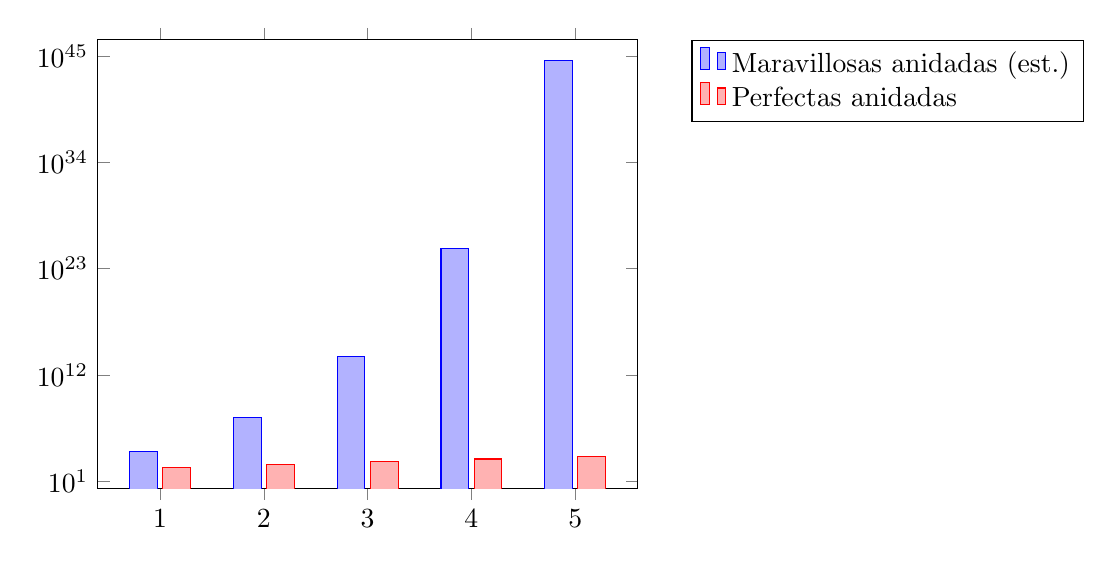
\begin{tikzpicture}
		\begin{axis}[
			x tick label style={
				/pgf/number format/1000 sep=},
			enlargelimits=0.05,
			legend style={at={(1.1,1)},
				anchor=north west},
			legend cell align={left},
			ybar,
			enlarge x limits={0.15},
			ymode=log,
		]
		\addplot 
			coordinates {(1,12870) (2,43705512) (3,8.83e13)
			(4,1.33e25) (5,3.68e44)};
		\addplot 
			coordinates {(1,256) (2,512) (3,1024)
			(4,2048) (5,4096)};
		\legend{Maravillosas anidadas (est.),Perfectas anidadas}
		\end{axis}
	\end{tikzpicture}
	\caption{Comparación entre la cantidad estimada de secuencias maravillosas
	anidadas y la cantidad de secuencias perfectas anidadas, para $m = 8$
	(escala logarítmica).}
	\label{figure:compare-marvellous-perfect}
\end{figure}

Aplicando esta misma metodología para otros valores de $m$ ($m = 4, 5, 6$),
observamos un comportamiento similar, con la cantidad estimada de secuencias
maravillosas anidadas aumentando muy rápidamente al incrementar $n$. En ningún
caso pudimos llegar a valores de $n$ mayores que $m$, menos aún estudiando
una porción lo suficientemente grande del espacio de búsqueda como para
verificar un posible declive en la cantidad de secuencias,
lo cual hubiera sido de interés para corroborar la validez de la primera de
nuestras conjeturas.

\chapter{Secuencias maravillosas anidadas, discrepancia y normalidad}

\begin{theorem}
\label{theorem:discrepancy-bound}
Sea $b > 0$, $\varphi$ una función creciente, y sea $\alpha \in [0, 1)$ un número real
tal que su escritura en base $b$ es
\[ .w_0w_1w_2\dots \]
donde cada bloque $w_k$ es una secuencia $(b^k, \varphi(b^k))$-maravillosa
anidada.

Si $\varphi = \ord(N)$, entonces $\alpha$ es un número normal en base $b$ y,
además,
\[ \discrepancy{N}(\lbrace \alpha b^n \rbrace)_{n\geq0} = \ord\left( \frac{\log^2(N)}{N} \right). \]
\end{theorem}

\begin{remark}
	Alternativamente, si se pide que los $w_k$ sean secuencias
	$(k, \varphi(k))$-maravillosas anidadas (con $k = 1, 2, \dots$),
	se tiene un resultado análogo pero
	con $\log^3(N)$ en lugar de $\log^2(N)$ en la expresión de la discrepancia
	(ver \cite{levin-discrepancy-estimate}).
\end{remark}

Notar que cada bloque $w_k$ tiene tamaño $\varphi(b^k)b^k$.
Definimos para cada $k = 0, 1, \dots$ la posición en que comienza el bloque
$w_k$, $s_k = \sum_{i=0}^k \varphi(i) b^i$.

\begin{lemma}
	\label{lemma:discrepancy-1}
	Sea $k$ un entero no negativo y sea $i$ tal que $1 \leq i \leq b^k$. Definimos
	\[ \alpha_{ki}(n) = \frac{[\lbrace \alpha b^{s_k + n} \rbrace b^i]}{b^i}, \]
	el número real que resulta de considerar $i$ dígitos de la expansión de
	$\alpha$ en base $b$, comenzando en la posición $s_k + n$.

	Sea $0 \leq S \leq \varphi(b^k)b^{k-i}$; para todo $f = 0, \dots, b^i$ tenemos que
	\[ \tilde{\mathbb{A}}_{ki}(S;f) = A\left(\frac{f}{b^i}, S \varphi(b^k) b^i, \varphi(b^k) b^i, \left(\alpha_{ki}(n)\right)_{n\geq0} \right) = \varphi(b^k)f + (i - 1)\varepsilon, \qquad \vert\varepsilon\vert \leq 1. \]
\end{lemma}

\begin{proof}
Si observamos la expresión
\[ A\left(\frac{f}{b^i}, S \varphi(b^k) b^i, \varphi(b^k) b^i, \left(\alpha_{ki}(n)\right)_{n\geq0} \right), \]
notamos
que se están considerando $\varphi(b^k)b^i$ mantisas de $\alpha$, comenzando
en la posición $s_k + S\varphi(b^k)b^i$, y truncando todas ellas a $i$ dígitos.
Consideremos por un lado el multiconjunto de estas mantisas,
\[ A_1 = \left\lbrace \alpha_{ki}(n) \;\Big\vert\; S \varphi(b^k) b^i \leq n < (S) \varphi(b^k) b^i \right\rbrace. \]

Por construcción, a partir de la posición $s_k$ la expansión decimal de
$\alpha$ contiene una secuencia $(b^k, \varphi(b^k))$-maravillosa anidada,
es decir, una concatenación de secuencias
$(i, \varphi(b^k))$-maravillosas anidadas. Cada una de estas secuencias tiene
longitud $\varphi(b^k)b^{i}$ y comienza en una posición congruente a $s_k$
módulo $\varphi(b^k)b^{i}$.

Esto quiere decir que las posiciones de inicio de todas las mantisas de $A_1$
caen dentro de una misma secuencia $(i, \varphi(b^i))$-maravillosa anidada.
Siendo $\beta_0, \beta_1, \dots, \beta_{\varphi(b^k)b^{i}-1}$ los caracteres
de dicha secuencia, consideremos el multiconjunto de los números reales cuya
parte fraccional, escrita en base $b$, se corresponde con una palabra de longitud
$i$ que aparece circularmente en ella:
\[ A_2 = \left\lbrace \sum_{j=0}^{i} \beta_{\ell \oplus j} b^{-j} \;\Bigg\vert\; \ell = 0, \dots, \varphi(b^k)b^i \right\rbrace, \]
donde $\oplus$ representa la suma módulo $\varphi(b^k)b^{i}$.

Podemos observar que los elementos de $A_2$ se corresponden exactamente con
los números reales $f'b^{-i}$ para $f' = 0, \dots, b^i$.
Además, recordemos que en una secuencia $(i, \varphi(b^i))$-maravillosa anidada,
cada palabra de longitud $i$ aparece exactamente $\varphi(b^k)$ veces.
Esta es, por lo tanto, la multiplicidad de cada uno de los elementos de $A_2$.
De aquí podemos concluir que
\[ \# \left\lbrace x \in A_2 \;\Big\vert\; x < \frac{f}{b^i} \right\rbrace = \varphi(b^k)f. \]

Por otra parte, $A_1$ y $A_2$ difieren en, a lo sumo, $i - 1$ elementos,
aquellos que se encuentran al final de la secuencia maravillosa anidada y
que, en el caso de $A_1$, se completan con dígitos de la secuencia siguiente,
mientras que en $A_2$ se completan circularmente con caracteres del comienzo.
Por lo tanto,
\begin{align*}
	A\left(\frac{f}{b^i}, S \varphi(b^k) b^i, \varphi(b^k) b^i, \left(\alpha_{ki}(n)\right)_{n\geq0} \right)
		&= \# \left\lbrace x \in A_1 \;\Big\vert\; x < \frac{f}{b^i} \right\rbrace \\
		&= \# \left\lbrace x \in A_2 \;\Big\vert\; x < \frac{f}{b^i} \right\rbrace + (i - 1)\varepsilon, & \vert\varepsilon\vert &\leq 1 \\
		&= \varphi(b^k)f + (i - 1)\varepsilon. && \qedhere
\end{align*}

\end{proof}

\begin{lemma}
	\label{lemma:discrepancy-2}
	Sea $\gamma \in [0, 1)$. Tenemos que
	\[ \mathbb{A}_{ki}(S;\gamma) =
		A\left(\gamma, S \varphi(b^k) b^i, \varphi(b^k) b^i, \lbrace \alpha b^{s_k + n} \rbrace_{n\geq0} \right) = \gamma\varphi(b^k)b^i + (\varphi(b^k) + i - 1)\varepsilon, \qquad \vert\varepsilon\vert \leq 1. \]
\end{lemma}

\begin{proof}
Sea $f = [\gamma b^i]$, de modo que $f = \gamma b^i - \varepsilon_1$, con
$\varepsilon_1 \in [0, 1)$. Notar que
\begin{align*}
	\tilde{\mathbb{A}}_{ki}(S;f) \leq \mathbb{A}_{ki}(S;\gamma) &\leq \tilde{\mathbb{A}}_{ki}(S;f+1).
\end{align*}
Reemplazando, según el Lema \ref{lemma:discrepancy-1}, tenemos que
\begin{align*}
	\varphi(b^k)f + (i - 1)\varepsilon_2 \leq \mathbb{A}_{ki}(S;\gamma) &\leq \varphi(b^k)f + \varphi(b^k) + (i - 1)\varepsilon_2.
\end{align*}
Por lo tanto,
\begin{align*}
	\mathbb{A}_{ki}(S;\gamma) &= \varphi(b^k)f + \varphi(b^k)\varepsilon_3 + (i - 1)\varepsilon_2, & \varepsilon_3 & \in [0, 1] \\
		&= \varphi(b^k)(\gamma b^i - \varepsilon_1) + \varphi(b^k)\varepsilon_3 + (i - 1)\varepsilon_2 \\
		&= \gamma\varphi(b^k)b^i + \varphi(b^k)(\varepsilon_3 - \varepsilon_1) + (i - 1)\varepsilon_2 \\
		&= \gamma\varphi(b^k)b^i + (\varphi(b^k) + i - 1)\varepsilon, & \vert\varepsilon\vert & \leq 1
\end{align*}
como queríamos demostrar.
\end{proof}

\begin{lemma}
	\label{lemma:discrepancy-3}
	Sea $\gamma \in [0, 1)$, y sea $1 \leq N \leq \varphi(b^k)b^{b^k}$. Tenemos que
	\[ A\left(\gamma, s_k, N, \lbrace \alpha b^{n} \rbrace_{n\geq0} \right) =
	\gamma N + \ord \left(b^{2k} + b^{k} \varphi(b^k) \right). \]
\end{lemma}

\begin{proof}
Comenzamos por observar las posiciones iniciales de las mantisas a considerar;
todas ellas están comprendidas entre las posiciones $s_k$ y $s_{k+1}$ del
desarrollo en base $b$ de $\alpha$, por lo que pertenecen a una misma
secuencia $(b^k, \varphi(b^k))$-maravillosa anidada.

Sea $N' = \left[ \frac{N}{\varphi(b^k)b} \right]$, y $N'' < \varphi(b^k)b$ de
forma tal que 
\[ N = N'\varphi(b^k)b + N''. \]
Sea $(N')_b = \nu_{b^k-2}\nu_{b^k-3}\dots\nu_0$
la escritura de $N'$ en base $b$. Para cada $i = 0, \dots, b^k-1$, sea
$N_i = \sum_{j=b^k-i-1}^{b^k-2} \nu_{j}b^{j} = (\nu_{b^k-2}\dots\nu_{b^k-i}\underbrace{0\dots0}_{b^k-2-i})_b$ el resultado de reemplazar por ceros los dígitos de la
escritura de $N'$ en base $b$ a partir del $i+1$-ésimo.
Notar que $0 = N_0 \leq N_1 \leq \dots \leq N_{b^k-1} = N'$.

Esto nos permite agrupar las $N$ mantisas a considerar en bloques consecutivos,
siguiendo los niveles de anidación de la secuencia maravillosa anidada:
\begin{itemize}
	\item Los primeros $b^k - 1$ bloques van desde la posición $N_{i+1}$ a la
		$N_{i}$, para $i = 1, \dots, b^k - 1$. Cada uno de ellos se corresponde
		exactamente con $\nu_{b^k-i-1}$ secuencias
		$(b^k - i, \varphi(b^k))$-maravillosas anidadas consecutivas.
	\item El último bloque va desde la posición $N'\varphi(b^k)b$ hasta la
		posición $N$. Comprende las últimas $N''$ mantisas, que no son suficientes
		para conformar una secuencia $(1, \varphi(b^k))$-maravillosa anidada.
\end{itemize}

Teniendo en cuenta lo anterior, podemos reescribir
\begin{align*}
	A(\gamma, &s_k, N, \lbrace \alpha b^{n} \rbrace_{n\geq0}) \\
	&= \sum_{i=1}^{b^k-1} A\left(\gamma, s_k + N_{i-1}\varphi(b^k)b, \nu_{b^k-i-1}\varphi(b^k)b^{b^k-i}, \lbrace \alpha b^{n} \rbrace_{n\geq0} \right) \\
	& \qquad + A\left(\gamma, s_k + N' \varphi(b^k)b, N'', \lbrace \alpha b^{n} \rbrace_{n\geq0} \right) \\
	&= \sum_{i=1}^{b^k-1} A\left(\gamma, N_{i-1}\varphi(b^k)b, \nu_{b^k-i-1}\varphi(b^k)b^{b^k-i}, \lbrace \alpha b^{s_k+n} \rbrace_{n\geq0} \right) + N''\varepsilon'', & \varepsilon'' &\in [0, 1].
\end{align*}

Sea, para cada $i = 1, \dots, b^k - 1$, $S_i = \frac{N_{i-1}}{b^{b^k - i - 1}}$.
Reemplazando en la expresión anterior, y reagrupando nuevamente las mantisas,
obtenemos
\begin{align*}
	&= \sum_{i=1}^{b^k-1} A\left(\gamma, S_i\varphi(b^k)b^{b^k-i}, \nu_{b^k-i-1}\varphi(b^k)b^{b^k-i}, \lbrace \alpha b^{s_k+n} \rbrace_{n\geq0} \right) + N''\varepsilon'' \\
	&= \sum_{i=1}^{b^k-1} \sum_{j=0}^{\nu_{b^k-i-1}-1} A\left(\gamma, (S_i + j)\varphi(b^k)b^{b^k-i}, \varphi(b^k)b^{b^k-i}, \lbrace \alpha b^{s_k+n} \rbrace_{n\geq0} \right) + N''\varepsilon'' \\
	&= \sum_{i=1}^{b^k-1} \sum_{j=0}^{\nu_{b^k-i-1}-1} \mathbb{A}_{k,b^k-i}(S_i+j; \gamma) + N''\varepsilon''.
\end{align*}

Finalmente, aplicando el Lema \ref{lemma:discrepancy-2},
\begin{align*}
&= \sum_{i=1}^{b^k-1} \sum_{j=0}^{\nu_{b^k-i-1}-1} \left( \gamma\varphi(b^k)b^{b^k-i} + (\varphi(b^k) + b^k - i - 1)\varepsilon_i \right) + N''\varepsilon'',
& \vert \varepsilon_i \vert & \leq 1 \\
&= \gamma\varphi(b^k) \sum_{i=1}^{b^k-1} \nu_{b^k-i-1}b^{b^k-i} + \sum_{i=1}^{b^k-1} (\varphi(b^k) + b^k - i - 1)b\varepsilon_i + N''\varepsilon'' \\
&= \gamma\varphi(b^k)b N' + \frac{1}{2}\left(b^{2k} - b^k + 2(b^k-1)\varphi(b^k) \right)b\varepsilon' + N''\varepsilon'',
& \vert \varepsilon' \vert & \leq 1 \\
&= \gamma N + \frac{1}{2}\left(b^{2k} - b^k + 2(b^k+1)\varphi(b^k) \right)b\varepsilon,
& \vert \varepsilon \vert & \leq 1. \\
&= \gamma N + \ord \left(b^{2k} + b^{k} \varphi(b^k) \right). && \qedhere
\end{align*}
\end{proof}

\begin{proof}[Demostración del Teorema \ref{theorem:discrepancy-bound}]

Para todo $N$, existe un entero $K$ tal que $N \in [s_K, s_{K+1})$, de forma
tal que $N = s_K + R$ con $0 \leq R < \varphi(b^K)b^{b^K}$.
Notar que $N \geq s_K \geq \varphi(b^{K-1})b^{b^{K-1}}$, por lo que
$b^K \leq b \log_b(N)$.
Agrupando las primeras
$N$ mantisas de $\alpha$ según el bloque al que corresponden, podemos escribir
\begin{align*}
A(\gamma, N, \lbrace \alpha b^n \rbrace_{n \geq 0})
	&= \sum_{k=0}^{K - 1} A(\gamma, s_k, \varphi(b^k)b^{b^k}, \lbrace \alpha b^n \rbrace_{n \geq 0})
		+ A(\gamma, s_K, R, \lbrace \alpha b^n \rbrace_{n \geq 0}) \\
	&= \sum_{k=0}^{K - 1} \left( \gamma \varphi(b^k)b^{b^k} + \ord \left(b^{2k} + b^{k} \varphi(b^k) \right) \right)
		+ \gamma R + \ord \left(b^{2K} + b^{K} \varphi(b^K) \right) \\
	&= \gamma N + \ord \left(\log^2(N) + \log(N) \varphi(\log(N)) \right).
\end{align*}

Dado que $\discrepancy{N}(\lbrace \alpha b^n \rbrace)_{n \geq 0} = \sup_{\gamma \in (0,1]} \left\vert N^{-1} A(\gamma, N, (\lbrace \alpha b^n \rbrace)_{n \geq 0}) - \gamma \right\vert$, resulta que

\[ \discrepancy{N}(\lbrace \alpha b^n \rbrace)_{n \geq 0} = \ord \left(\frac{\log^2(N) + \log(N) \varphi(\log(N))}{N} \right). \]

Concretamente, si $\varphi = \ord(N)$, tenemos que $\varphi(\log(N)) = \ord(\log(N))$, y por lo tanto,
\[ \discrepancy{N}(\lbrace \alpha b^n \rbrace) = \ord \left( \frac{\log^2(N)}{N} \right). \qedhere \]
\end{proof}
